%%This is a very basic article template.
%%There is just one section and two subsections.
\documentclass{article}

\usepackage{iclr2016_conference,times}
\usepackage{amsmath}
\usepackage{amsfonts}
\usepackage{parskip}
\usepackage{subcaption}
\usepackage{xcolor} 
\usepackage{cleveref}
\usepackage{tikz}
\usepackage{pgfplots}
\usepackage{algorithm}
\usepackage{algpseudocode}
\usepackage{graphicx}
\newcommand{\indep}{\rotatebox[origin=c]{90}{$\models$}}
\DeclareMathOperator*{\argmin}{argmin}
\title{\LARGE{Pattern as a Foreign Language} \\ \large{TTIC 31210 Project Report \\ Spring 2017}}

\author{Hao Jiang \\ The University of Chicago}
\begin{document}

\maketitle

\begin{abstract}
The recurrent neural network (RNN) based encoder-decoder architecture has been widely used for various sequence-to-sequence translation tasks such as natural language translation and grammar inference, and has achieved significant success on these tasks. In this project, we attempt to use this architecture to infer common patterns from multiple inputs, which is a crucial task for information extraction and management. This leads to two new types of tasks: combinations and summarization. In combination task, we train the encoder-decoder with known patterns and attempt to use it to recognize the combination of these patterns. In summarization task, we define some rules to infer a common pattern from multiple records and use encoder-decoder to learn these rules. Preliminary results show that existing architecture does NOT fit these applications and new architectures are required.
\end{abstract}

\section{Introduction}
In this project, we explore the possibility of using RNN-based encoder-decoder architecture to do pattern extraction. Pattern extraction infers common patterns from multiple records, and extract sub-components from the records accordingly. \Cref{fig:pattern} demonstrates several lines of Java application logs and the pattern inferred from them. Pattern extraction allows in-depth understanding of the data's nature, enabling more efficient data compression and accurate data analysis. Previous methods of pattern extraction developed by \cite{dirt_2008} use a rule-based method to iteratively extract common words from records, which is inefficient when dealing with large dataset. In addition, this method does not learn from past dataset to speed up future processing. We plan to use RNN to address these problems.

Recurrent neural network(RNN) based encoder-decoder architecture has recently been widely adopted in various tasks such as neural machine translation (\cite{ntran_2013, rnned_2014}), image captioning (\cite{icap_2015} and grammar inference (\cite{grammar_2014}). These tasks can all be viewed as a translation between source and target domains using encoding-decoding process. First, an encoder is employed to convert the input to a single vector, which is supposed to contain a summary of the input. With that encoded state as input, a decoder is then used to generate an output belonging to the destination domain from the encoded result. The entire encoder-decoder model is trained on  source-target pairs to maximize the probability of correct translation.

A potential challenge of using RNN encoder for pattern extraction is constructing an efficient training set. Unlike in the case of natural language and grammar, the pattern does not have a closed, well-defined domain. The vocabularies of pattern can be arbitrary combinations of alphabet, numbers and symbols. There's also no ``grammar'' governing these vocabularies. Thus the attempt to construct a complete training set that covers all possible patterns is infeasible. Instead, we try to attack the problem from different directions.

In this project, we experiment with two approaches. First, we attempt to imitate human's ability to recognize some common pattern, e.g., date, time and ip address. We train the encoder-decoder model with these common patterns, and explore the model's ability to recognize combination of these patterns. This method will allow the model to remember some patterns and recognize them when later encounter these pattern again. Second, we develop an architecture allowing multiple inputs to be encoded into a single state, and use this model to train on a dataset containing inputs and patterns inferred from them, in order to evaluate the ability of RNN-based encoder-decoder on directly inferring patterns from multiple inputs. In the experiment, we notice that none of these methods give a satisfied result on the topic, which implies that traditional RNN-based encoder-decoder architecture is not suitable for such kind of tasks and new architecture is needed. 

The remainder of the paper is organized as following. \Cref{sec:background} introduce the pattern extraction problem and RNN-based encoder-decoder structure, including previous works. \Cref{sec:pernn} describes the method we experiment with in this report. \Cref{sec:experiment} demonstrates the experiment result and \Cref{sec:conclusion} conclude our finding.

\begin{figure}
\centering
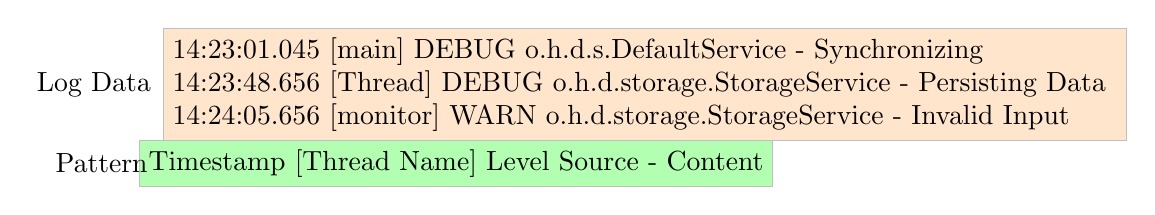
\begin{tikzpicture}
\node[text width=12cm, draw=lightgray, fill=orange!20] (a){
14:23:01.045 [main] DEBUG o.h.d.s.DefaultService - Synchronizing \\
14:23:48.656 [Thread] DEBUG o.h.d.storage.StorageService - Persisting Data \\
14:24:05.656 [monitor] WARN o.h.d.storage.StorageService - Invalid Input \\
};
\node[below of =a,draw=lightgray,fill=green!30,xshift=-2.4cm](b){Timestamp [Thread Name] Level Source - Content};
\node[left of =a, xshift = -6cm]{Log Data};
\node[left of = b,xshift=-3.5cm]{Pattern};
\end{tikzpicture}
\caption{Application Log and extracted Pattern}
\label{fig:pattern}
\end{figure}

\section{Background}\label{sec:background}
\subsection{Pattern Extraction}
Most data management systems are designed to process organized, structural data. However, many real-world datasets that contain valuable information do not belong to this category. Examples include system logs, documents and image files. To manage these datasets with existing dbms, one important step is to organize these non-structual or semi-structual datasets into structual format. However, this task is challenging as these datasets often come missing documentation or with incomplete descriptions. Thus automatic inferrence of structure hidden in dataset  is crucial to efficient processing of ad hoc data. This task is called pattern extraction.

The state-of-art research regarding pattern extraction from textual data is described in \cite{dirt_2008}. The authors defined a domain language to describe pattern for non-structual data, and proposed a rule-based algorithm to discover common patterns from a list of textual records. The algorithm first locate frequently appeared symbols (for example, the ``:'' in a timestamp record or ``.'' in IP address) from these records, and use them to split the records into smaller group of pieces. The process is repeated untill no common symbol can be found. The algorithm considers each group of pieces as a union of tokens, and apply various rules to abstract the structure. Based on the idea, software systems such as \cite{pads,recbreaker} are built and put into practice. 

\subsection{RNN based encoder-decoder architecture}
Traditional feed-forward neural network can only process input of fixed size, which makes it infeasible for variable length input such as textual and speech data. Recurrent neural network (\cite{rnn_1988, rnn_1990}) overcomes this limitation by concatenating multiple neural networks sharing same parameters together, with each network corresponds to a single input in the input sequence. However, in this setting, RNN will always output a sequence that has the same length of the input. To perform translation between sequences of different length, \cite{rnned_2014} proposed a RNN-based encoder-decoder architecture, in which a RNN is used to encode input sequence as a fixed-length vector (the encoded state), and another RNN is used to expand this encoded state into the output sequence. This structure  is shown in \Cref{fig:rnn}. 

\begin{figure}
\centering
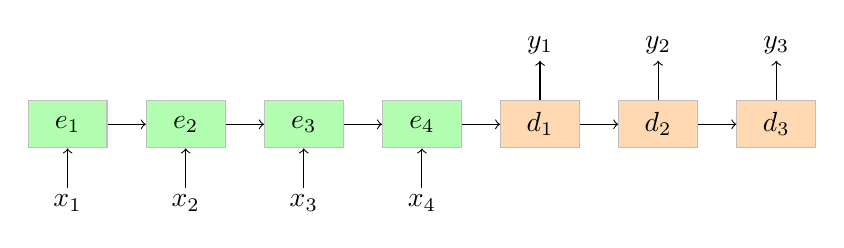
\begin{tikzpicture}[
encell/.style={draw=lightgray,fill=green!30, minimum width=1cm, minimum height=0.6cm},
decell/.style={draw=lightgray,fill=orange!30, minimum width=1cm, minimum height=0.6cm}
]
\node[encell](ea) at (-4.5,0) {$e_1$};
\node[encell](eb) at (-3,0) {$e_2$};
\node[encell](ec) at (-1.5,0) {$e_3$};
\node[encell](ed) at (0,0) {$e_4$};

\node[decell](da) at (1.5,0) {$d_1$};
\node[decell](db) at (3,0) {$d_2$};
\node[decell](dc) at (4.5,0) {$d_3$};

\node at (-4.5,-1){{$x_1$}};
\draw [->]([yshift=-0.5cm]ea.south) to (ea.south);
\node at (-3,-1){{$x_2$}};
\draw [->]([yshift=-0.5cm]eb.south) to (eb.south);
\node at (-1.5,-1){{$x_3$}};
\draw [->]([yshift=-0.5cm]ec.south) to (ec.south);
\node at (0,-1){{$x_4$}};
\draw [->]([yshift=-0.5cm]ed.south) to (ed.south);


\draw[->](ea) to (eb);
\draw[->](eb) to (ec);
\draw[->](ec) to (ed);


\draw[->](ed) to (da);
\draw[->](da) to (db);
\draw[->](db) to (dc);


\node at (1.5,1){{$y_1$}};
\draw [->](da.north) to ([yshift=0.5cm]da.north);
\node at (3,1){{$y_2$}};
\draw [->](db.north) to ([yshift=0.5cm]db.north);
\node at (4.5,1){{$y_3$}};
\draw [->](dc.north) to ([yshift=0.5cm]dc.north);

\end{tikzpicture}
\caption{Recurrent Neural Network based Encoder-Decoder}
\label{fig:rnn}
\end{figure}


\cite{s2snn_2014} adopts Long Short-Term Memory (LSTM, \cite{lstm_1997}) in this architecture for machine translation. Later, variants of this network such as Attention (\cite{attention_2015}) are also proposed for an improved accuracy. In \cite{grammar_2014}, the authors demonstrated that LSTM-based auto encoders can be used to infer tree-like structures such as grammars from sequential input, which also inspires us to propose the idea described in this report.

\section{Pattern Extraction with RNN}\label{sec:pernn}
\subsection{Pattern Combination}\label{sec:combo}

\subsection{Pattern Inferrence}\label{sec:pattern}

\section{Experiment}\label{sec:experiment}

\section{Conclusion}\label{sec:conclusion}

\bibliographystyle{iclr2016_conference}
\bibliography{ref}
\end{document}
